\documentclass[11pt]{article}
\usepackage{graphicx}
\usepackage{float}
\usepackage{amsmath}
\usepackage[a4paper,width=150mm,top=25mm,bottom=25mm,bindingoffset=6mm]{geometry}
\usepackage{fancyhdr}
\usepackage{multirow}
\usepackage{caption}
\usepackage{subcaption}
\usepackage[table,xcdraw]{xcolor}
\usepackage{url}
\pagestyle{fancy}
\fancyhead{}
\fancyhead[RO,LE]{Movie Recommendation System}
\usepackage[document]{ragged2e}

% \fancyfoot{}
% \fancyfoot[LE,RO]{Page:\thepage}


\begin{document}

\begin{titlepage}
    \begin{center}
        \vspace*{1cm}
        
        \Huge
        \textbf{Movie Recommendation System}
        
        \vspace{0.5cm}
        \LARGE
        ECS 171 Machine Learning
        
        \vspace{0.5cm}
        \LARGE
        Group 29 Project Report

        
        \vspace{1.5cm}
        \textbf{Group Members:}
        
        \vspace{0.5cm}
        Sizhuo Sun, Wilson Lu, Jashanpreet Singh, Andrew Lam
        
        \vspace{1.5cm}
        \textbf{Github Repository:}

        \vspace{0.5cm}
        https://github.com/hungry5656/movie-recommender-system
        
        \vfill
        
    \end{center}
\end{titlepage}

\large

    \begin{flushleft}
        \textbf{\LARGE Introduction and Background}
    \end{flushleft}

\vspace{0.3cm}
\justifying
Movies are one of the largest forms of consumed media in modern times. They serve to provide entertainment and comfort for people who need to kick back and relax from their usually busy schedule. It’s because of this there is a large demand for newer and high quality movies for people to watch. To combat this problem there are a few solutions that could be considered. For one a consumer could just continue to watch random movies without considering if the movie is for them or not, leaving them with a more than likely lesser experience as opposed to watching a movie that was specifically identified with what the person liked. Being able to figure out and recommend movies that a person would like is paramount to keeping viewer engagement while also keeping them happy and comfortable.

\vspace{0.3cm}

That’s where machine learning models come in. They are able to analyze users and give them recommendations based on their own preferences. Not only can they give recommendations based on the user but also movies that other users have recommended. There is not much room for data to skew or have complex nuances, so error will not be very high and conversely accuracy will be high.

\vspace{0.3cm}

There are already many instances of these models being put to work in the real world. Although there are not many fields where these movie recommendation systems can be applied, the general idea of a recommendation system can be almost universal. For example:

\vspace{0.3cm}

    \begin{itemize}
        \item Netflix:
        \begin{itemize}
            \item Netflix utilizes a recommendation systems that starts with the users base impressions and preferences and recommends based on those preferences. As the user watches more movies/shows, those preferences are slowly changed to recommend movies/shows based on what they are watching and not just based on the users preferences
        \end{itemize}
    \end{itemize}
	

\vspace{0.3cm}

This is how it is for most Movie/Show based platforms and it also extends to video sharing platforms.

\vspace{0.3cm}

    \begin{flushleft}
        \textbf{\LARGE Literature review}
    \end{flushleft}

\vspace{0.3cm}

Machine Learning has a big presence when it comes to recommendation systems, especially for areas such as movies in the entertainment industry. Research is constantly being done on how to predict an accurate recommendation, as there often is no fine classification or answer to a good recommendation. Below is an example of previous movie recommendation model systems that have been implemented using a variety of techniques.
\vspace{0.3cm}

A group of computer scientists (M. Chenna Keshava, P. Narendra Reddy, S. Srinivasulu, and B. Dinesh Naik) did research into which model that was used would produce the best results in terms of movie recommendations. The dataset that they used was the Netflix Prize data which was taken from Kaggle, and the models that were tested consisted of XGBoost, Surprise BaselineOnly, Surprise KNNBaseline, Matrix Factorization SVD, and Matrix Factorization SVDpp. Their conclusion showed that their best model for movie recommendations was SVDpp with a test RMSE of 1.0675, which was the lowest among the other four models that were used. The authors also noted that they could have gained better results by tuning hyperparameters or by using the full dataset.

\vspace{0.3cm}

In a different study, Raja Marappan and S. Bhaskaran presented a few approaches to studying the accuracy of other models, such as content-based, collaborative-based, and cosine similarity approach to recommending movies. With their implementations of their model, they concluded that cosine similarity gave the best results when assessing the speed and accuracy compared to other models. 
\vspace{0.3cm}
The different approaches to choosing a model, along with the RMSE reporting, were a good reference point for how we constructed and evaluated our model.

\vspace{0.5cm}

    \begin{flushleft}
        \textbf{\LARGE Dataset Description and Exploratory Data Analysis of the data set}
    \end{flushleft}


The Movies Dataset is a comprehensive collection of metadata and ratings for over 45,000 movies. It provides valuable information for various analyses and modeling tasks. The dataset consists of several files, including \texttt{movies\_metadata.csv}, \texttt{keywords.csv}, \texttt{credits.csv}, \texttt{links.csv}, \texttt{links\_small.csv}, and \texttt{ratings\_small.csv}. In our model, we focused on \texttt{movies\_metadata.csv} and \texttt{ratings\_small.csv}.

\vspace{0.3cm}

\texttt{movies\_metadata.csv} contains features such as movie titles, release dates, genres, production companies, languages, budget, revenue, and \texttt{movieId}, among others. Each row represents a movie, and the columns provide detailed information about the movie's characteristics.

\vspace{0.3cm}

\texttt{ratings\_small.csv} consists of 45,000 ratings on a scale of 1-5, given by 671 unique users. These ratings were obtained from the official GroupLens website. The ratings dataset includes the \texttt{movieId} but does not include the movie title, which is why we need the metadata dataset for that information. This subset of data is useful for exploring user ratings and building recommendation systems.

\vspace{0.3cm}

To prepare the data for analysis, we dropped all columns from the \texttt{movies\_metadata} dataset except for the \texttt{movieID}. We kept the \texttt{ratings\_small.csv} dataset as is. Then, we merged the two datasets based on the \texttt{movieID} column. We removed any \texttt{NaN} values from the merged dataset. The final result is a cleaned dataset that looks like the following: 

\vspace{0.3cm}

\begin{figure}[H]
  \centering
  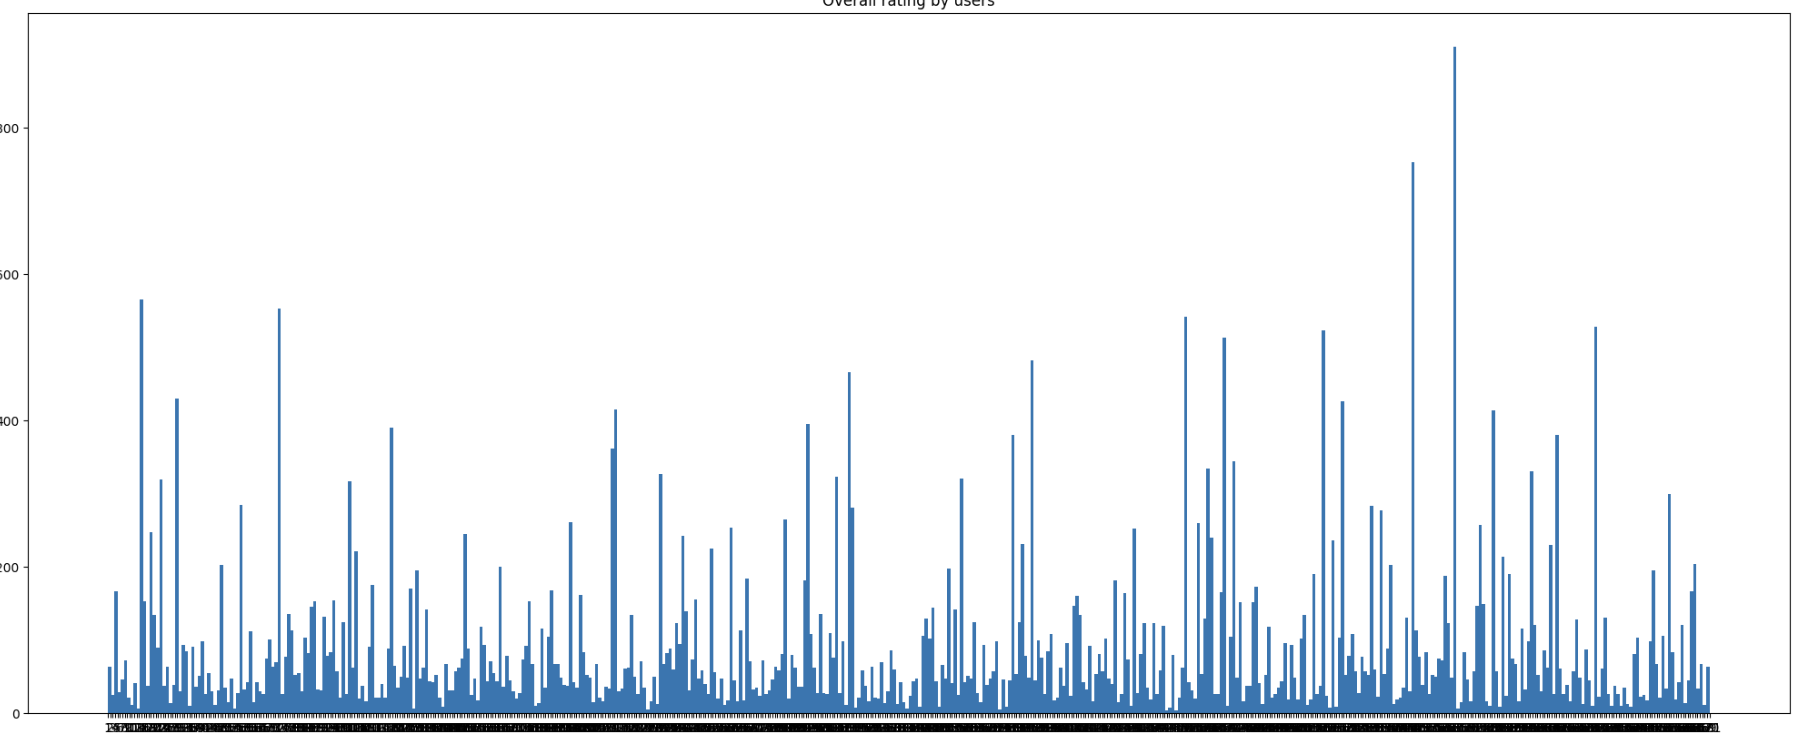
\includegraphics[width=0.8\textwidth]{image/ratings.png}
  \caption{Distribution of ratings}
\end{figure}

\vspace{0.3cm}

The histogram plot displays the distribution of user IDs across 500 bins, providing insights into the spread of user IDs in the dataset. By examining the histogram, we can assess whether the user IDs are evenly distributed or if there are any noticeable gaps in the distribution. Each bar's height in the histogram represents the frequency or count of user IDs falling within a specific range or bin.

This histogram allows us to identify outliers or peculiar patterns in the distribution of user IDs. Outliers are data points that significantly deviate from the general pattern, and they can be identified as bars that are notably higher or lower than the surrounding bars. In this particular dataset, we observe outliers where certain movies have received more than 800 ratings.

Analyzing the histogram aids in understanding the overall distribution of user IDs and provides insights into any exceptional cases or irregularities in the dataset.

\begin{figure}[H]
  \centering
  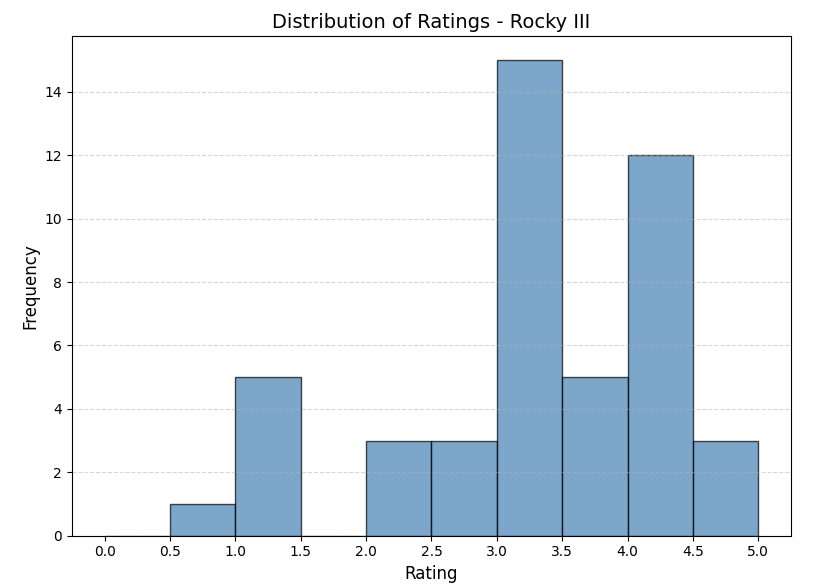
\includegraphics[width=.9\textwidth]{image/barplot.png}
  \caption{Barplot}
\end{figure}

The bar plot above specifically examines the ratings distribution for the movie \textbf{"Rocky III"}. It offers a visual representation of how the ratings are spread across various rating values for this particular movie. From the plot, it is evident that a significant portion of users gave it ratings of 3 and 4. The code in the notebook can be modified to investigate the distribution for any other movie in the dataset. By altering the movie name in the code, we can generate a tailored histogram plot that focuses on the ratings distribution for the selected movie. This flexibility allows for the exploration of specific movies within the dataset and provides insights into how users rate them.

\vspace{0.5cm}

    \begin{flushleft}
        \textbf{\LARGE Proposed Methodology}
    \end{flushleft}

After we did the data analysis for our dataset, there is a big problem for us to start the first step as all of us have little knowledge about recommendation system. We found a crash course about recommendation system at google developer website. By checking that crash course, we choose collaborative filter as the main method for our model as it is more suitable to find the relation between history data and connection between different users.

\vspace{0.3cm}

The main method we used is a Hybrid model which includes a retrieval model and a ranking model. A retrieval model is used as a binary decision model to filter the movies interested by user, and we use a basic two tower model here with a user embedding and movie embedding. We found a python library TensorFlow-recommender that have API specifically for retrieval and ranking model. As for how the data is represented in our model, we found an important method called matrix factorization that is widely used in recommendation system. As we learned from a paper about matrix factorization by Yehuda Koren, Robert Bell and Chris Volinsky, the input can be two embedding vector for user and movie with a dimension number n. The benefit for matrix factorization is that the product of user embedding vector and transpose of movie embedding is the feedback matrix, which can also be called as index matrix. This matrix have all the information between one user and movie so that we can extract those information to recommend movies. Embedding number defines the hidden attributes used by model to categorize different movies.

\vspace{0.3cm}

A ranking model is used to predict the rating for an unseen movie from a specific model. We used a DNN here to focus on predicting the rating for an unseen movie. One big problem to consider here is the hyperparameter tuning for this DNN as there are many combination of hyperparameters. The loss function is the combination of both loss information from retrieval model and ranking model. We use MSE as the loss function for ranking model and the default loss function for retrieval model. We add two weight parameter for ranking loss and retrieval loss so that we can evaluate how each model is performed individually. Here is a graph that shows how our model is structured.

\begin{figure}[H]
    \centering
    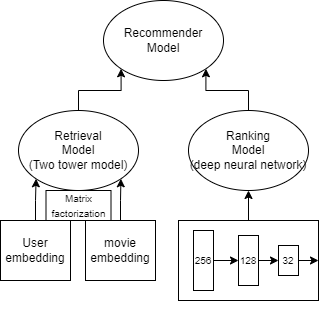
\includegraphics[width=.5\textwidth]{image/model_details.png}
    \caption{model details}
  \end{figure}

\vspace{0.5cm}

    \begin{flushleft}
        \textbf{\LARGE Experimental Result}
    \end{flushleft}

We have two parameters that can determine the portion between retrieval model and ranking model. We firstly train the two sub model individually to compare with how each model performed and what is been affected by each model. The method we use to evaluate our model is by using RMSE and MAE that is explained in chapter Recommender Systems Handbook: Evaluating recommendation systems written by Guy Shani and Asela Gunawardana. As there are limited option to evaluate recommender model, we found there is a built-in method used in tensorflow-recommender library called top\_k\_categorical\_accuracy. This value represents the percentage of the movies recommended by the system is in the top list for user. With the little attributes about movies we used and the naïve feature of recommender system, it is hard to get a close to one accuracy.

\vspace{0.3cm}

Since our model is not a traditional classification model, it is hard to implement grid search method to find the optimal set for hyperparameters. We manually tested possible values for each hyperparameters. We found out that learning rate being 0.2 is the best as higher value leads to an overfitting and lower value trains slowly. We tested different set of neural networks inside ranking model and get the combination of 256 * 128 * 32 has the balance between performance and training time. We found out that the relu activation function suits the best as our model only dealing with positive number from zero to one. The most important hyperparameter of our model is embedding dimension as it determines how many of different hidden attributes is seen by model. As we tested different numbers of embedding, larger number means a higher accuracy, but the drawbacks are potential overfitting and longer time to train a model. Due to the limitation of our hardware specification and time, we end up chose 64 as the number of embedding dimensions.

\begin{figure}[H]
    \centering
    \begin{subfigure}[b]{.45\textwidth}
        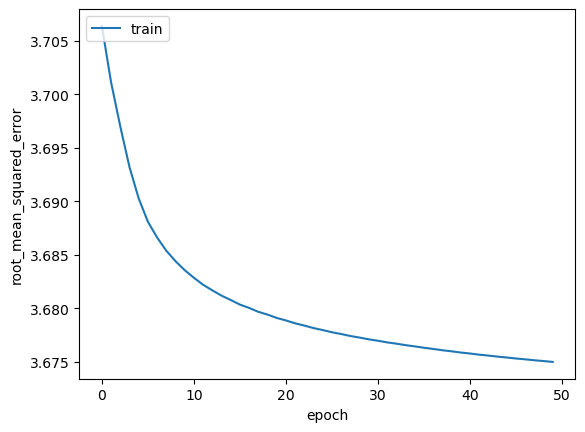
\includegraphics[width=\textwidth]{image/rmse.png}
        \caption{Root Mean Squared Error}
    \end{subfigure}
    \hfill
    \begin{subfigure}[b]{.45\textwidth}
        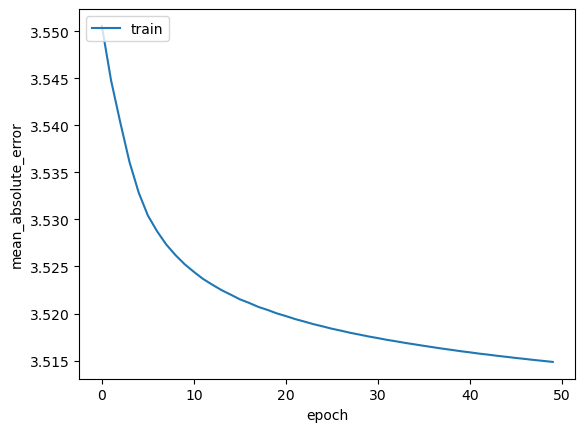
\includegraphics[width=\textwidth]{image/mae.png}
        \caption{Mean Absolute Error}
    \end{subfigure}
    \caption{Plots for different metrics and number of epochs}
  \end{figure}

  \begin{figure}[H]
    \centering
    \begin{subfigure}[b]{.45\textwidth}
        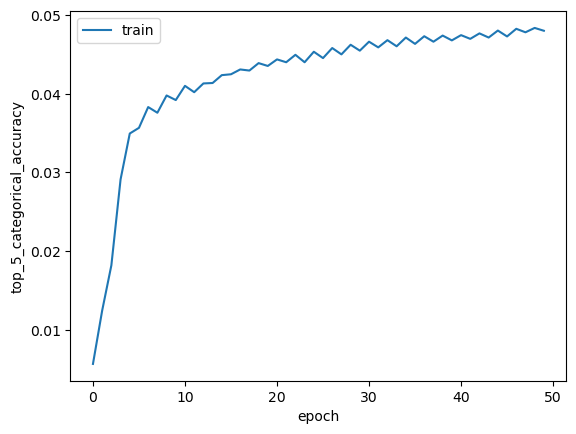
\includegraphics[width=\textwidth]{image/top5accuracy.png}
        \caption{top 5 accuracy}
    \end{subfigure}
    \hfill
    \begin{subfigure}[b]{.45\textwidth}
        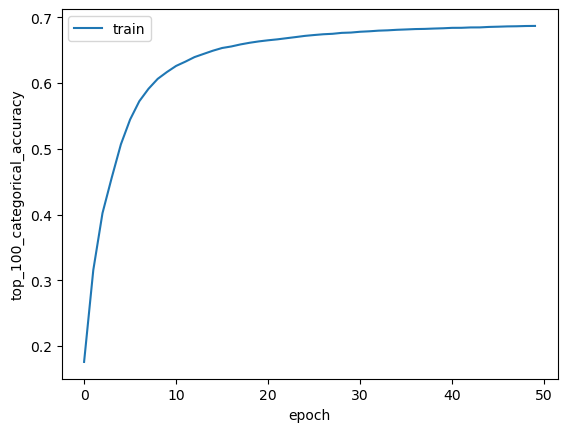
\includegraphics[width=\textwidth]{image/top100accuracy.png}
        \caption{top 100 accuracy}
    \end{subfigure}
    \caption{Plots for different metrics and number of epochs}
  \end{figure}

As shown in the two plots above, the improvement of root mean square error and mean absolute error is limited due to the small size of dataset. However, the accuracy has a big improvement for both top 5 selection and top 10 selection. The two plots for accuracy look like log function and rate to converge slows down as the number of epochs goes up. The table below shows the performance on the unseen data for the three types of model defined by how many weights each sub model has. The testing dataset and training dataset are split by the general dataset. The portion of training dataset and testing dataset is 80:20. We are using the evaluation API from TensorFlow to test our model in the testing set. The value we got from testing dataset is much lower than the training dataset as the nature of unsupervised learning. 

\begin{table}[H]
\centering
\begin{tabular}{|l|l|l|l|} 
\hline
Metrics                         & Mixed Model & retrieval Model & Ranking Model \\ 
\hline
root\_mean\_squared\_error      & 3.569873    & 3.866569        & 3.754806      \\ 
\hline
mean\_absolute\_error           & 3.413906    & 3.727047        & 3.613183      \\ 
\hline
top\_1\_categorical\_accuracy   & 0.000111    & 0.000000        & 0.000000      \\ 
\hline
top\_5\_categorical\_accuracy   & 0.002556    & 0.002556        & 0.000333      \\ 
\hline
top\_10\_categorical\_accuracy  & 0.006224    & 0.005446        & 0.000556      \\ 
\hline
top\_50\_categorical\_accuracy  & 0.027673    & 0.025006        & 0.000889      \\ 
\hline
top\_100\_categorical\_accuracy & 0.054679    & 0.050567        & 0.001889      \\
\hline
\end{tabular}
\caption{Testing results for Different sets of weights}
\end{table}

By comparing the data from the table above, the retrieval model has a higher top k accuracy whereas ranking model have a lower root mean squared error and mean absolute error. This means that retrieval model is good at selecting the related movies, and the ranking model is good at predicting the correct ratings, which follows the initial description of these two models. The mix of these two models combine the benefit from both. As shown in the table, the top k accuracy and the RMSE as well as MAE tend to be higher than either one of the model individually. 

\vspace{1cm}

    \begin{flushleft}
        \textbf{\LARGE Software Implementation}
    \end{flushleft}

\vspace{0.3cm}

Upon creating our collaborative-based recommendations model, we implemented a Flask website to deploy our system. Given an input of either a specific movie or a user id, our model will return a list of movies. 

\vspace{0.3cm}

Our UI contains a simple implementation where the user is given the option of either entering a user id or the name of a movie. Based on what the user inputs, our model will go through a collaborative filtering process based on user history and rating and return a list of 5 movie recommendations the user would be most interested in.

\vspace{0.3cm}

For our future implementation, we want to combine collaborative-based and content-based models to gain even more accurate results. We might implement this by having users enter their user id and adding another area where they can list their favorite directors, actors, or genres and return a list of that result. Another feature we could implement is having the user decide how many recommendations they want as; currently, the user gets a set of 5 movie recommendations with each input.

\vspace{1cm}

    \begin{flushleft}
        \textbf{\LARGE Conclusion}
    \end{flushleft}

In conclusion, movie recommendation systems play a crucial role in providing personalized and engaging movie suggestions to users based on their preferences. In this field, machine learning algorithms like collaborative filtering have been widely applied, enabling services like Netflix to provide consumers with personalized recommendations. As shown by the literature review and exploratory data analysis described, the study and use of movie recommendation systems have shown promising outcomes. There is still opportunity for advancement and additional application, though.

\vspace{0.3cm}

One potential area for improvement is the incorporation of hybrid models that combine collaborative filtering with content-based approaches. By considering both user preferences and movie attributes such as genres, directors, and actors, the recommendations can be more comprehensive and accurate. Additionally, utilizing deep learning techniques like neural networks could enhance the ranking and prediction models, providing better insights into users' movie preferences.

\vspace{0.3cm}

The introduction of hybrid models, which fuse collaborative filtering with content-based methods, is one possible avenue for improvement. The recommendations can be more thorough and precise if they take into account both user preferences and movie characteristics like genres, directors, and actors. The rating and prediction models may also be improved by using deep learning techniques like neural networks, which would provide customers more insights into their movie tastes. Additionally, increasing the dataset and adding more varied movie information, such user reviews, could increase the precision of the recommendations. The recommendation algorithm could be improved by including sentiment analysis methods to comprehend users' feelings toward movies.

\vspace{0.3cm}

In summary, by integrating hybrid models, leveraging advanced machine learning techniques, expanding the dataset, and incorporating real-time feedback, we can enhance the accuracy, personalization, and user satisfaction of movie recommendations in the future.

\pagebreak

\begin{center}
    \textbf{\LARGE References}
\end{center}
\begin{flushleft}

\textbf{\large Dataset:}

\vspace{0.3cm}
\url{https://www.kaggle.com/datasets/rounakbanik/the-movies-dataset}

\vspace{0.3cm}
\textbf{\large Recommendation System:}

\vspace{0.3cm}
\url{https://developers.google.com/machine-learning/recommendation}

\vspace{0.3cm}
\textbf{\large Literature review:}

\vspace{0.3cm}
Keshava, M. C., Srinivasulu, S., Reddy, P. N., \& Naik, B. D. (2020). Machine learning model for movie recommendation system. Int. J. Eng. Res. Tech, 9, 800-801.

\vspace{0.3cm}

Marappan, R., \& Bhaskaran, S. (2022). Movie recommendation system modeling using machine learning. International Journal of Mathematical, Engineering, Biological and Applied Computing, 12-16.

\vspace{0.3cm}
\textbf{\large Proposed Methodology:}

\vspace{0.3cm}
Koren, Y., Bell, R., \& Volinsky, C. (2009). Matrix factorization techniques for recommender systems. Computer, 42(8), 30-37.

\vspace{0.3cm}
\textbf{\large Experimental Result:}

\vspace{0.3cm}
Shani, G., \& Gunawardana, A. (2011). Evaluating recommendation systems. Recommender Systems Handbook, Ricci, F, Rokach, L, Shapira, B, and Kantor, PB, ed, 257-297.

\end{flushleft}
    

\end{document}